%%%%%%%%%%%%
%
% $Autor: Wings $
% $Datum: 2019-03-05 08:03:15Z $
% $Pfad: TemplateSensor $
% $Version: 4250 $
% !TeX spellcheck = en_GB/de_DE
% !TeX encoding = utf8
% !TeX root = filename 
% !TeX TXS-program:bibliography = txs:///biber
%
%%%%%%%%%%%%

% Structure
\chapter{CNC Shield V3}

\section{Einleitung}

Das CNC Shield V3 dient zur einfachen Ansteuerung mehrerer Schrittmotoren über einen Arduino Uno. 
Es wird direkt auf den Arduino aufgesteckt und stellt Steckplätze für Schrittmotortreiber sowie Anschlüsse für Motoren, Endschalter und weitere CNC-Funktionen bereit.

Im Projekt wird das CNC Shield V3 zur Ansteuerung der Achsmotoren des CNC-Hot-Wire-Foam-Cutters verwendet. 
Die Schrittmotoren bewegen den Heizdraht entlang der gewünschten Kontur. 
Dadurch ist das Shield eine zentrale Schnittstelle zwischen dem Arduino Uno, den Motortreibern und den mechanischen Achsen.

CNC-Systeme werden allgemein eingesetzt, um Bewegungen von Werkzeugen oder Werkstücken rechnergestützt und reproduzierbar auszuführen. 
Dabei werden Bewegungsdaten in Steuersignale für die Achsantriebe umgesetzt \cite{Hehenberger:2020}.

\section{Grundlagen}

Ein CNC Shield erweitert den Arduino Uno um Anschlüsse und Steckplätze, die für kleinere CNC-Anwendungen benötigt werden. 
Der Arduino übernimmt dabei die Erzeugung der Steuersignale. 
Das Shield verteilt diese Signale auf die einzelnen Achsen und stellt die Verbindung zu den Schrittmotortreibern her.

Für die Bewegung der Achsen werden Schrittmotoren verwendet. 
Die eigentliche Leistungsansteuerung übernimmt nicht das CNC Shield selbst, sondern der jeweilige Schrittmotortreiber. 
Das Shield stellt dafür die STEP-, DIR- und ENABLE-Signale bereit. 
Über das STEP-Signal werden Schrittimpulse erzeugt, über das DIR-Signal wird die Drehrichtung festgelegt und über ENABLE werden die Motortreiber aktiviert oder deaktiviert.

Das CNC Shield V3 ist für den Einsatz mit steckbaren Motortreibermodulen wie dem A4988 oder kompatiblen Treibern vorgesehen. 
Die Motortreiber werden auf die dafür vorgesehenen Steckplätze des Shields gesetzt. 
Dadurch können die einzelnen Achsen X, Y, Z und A separat angesteuert werden \cite{JoyIT:CNCShield:Anleitung}.

\section{Spezifischer CNC-Shield}

Im Projekt wird ein CNC Shield V3 für Arduino verwendet. 
Das Shield wird auf einen Arduino Uno gesteckt und dient als Verbindungsebene zwischen Mikrocontroller, Schrittmotortreibern und Schrittmotoren. 
Es besitzt Steckplätze für bis zu vier Motortreiber und kann dadurch mehrere Achsen eines kleinen CNC-Systems ansteuern \cite{JoyIT:CNCShield:Datenblatt}.

Für das Projekt werden insbesondere die Achsausgänge des Shields genutzt. 
Die Achsen bewegen den Heizdraht beziehungsweise den Schneidrahmen entlang der programmierten Bahn. 
Die Bewegung muss gleichmäßig erfolgen, damit der Draht das Material sauber schneiden kann.

Das Shield stellt außerdem Anschlüsse für Endschalter bereit. 
Diese können für Referenzfahrten oder zur Begrenzung der Achsbewegungen verwendet werden. 
Dadurch kann das System sicherer betrieben und eine definierte Ausgangsposition angefahren werden.

\begin{figure}[htbp]
	\centering
	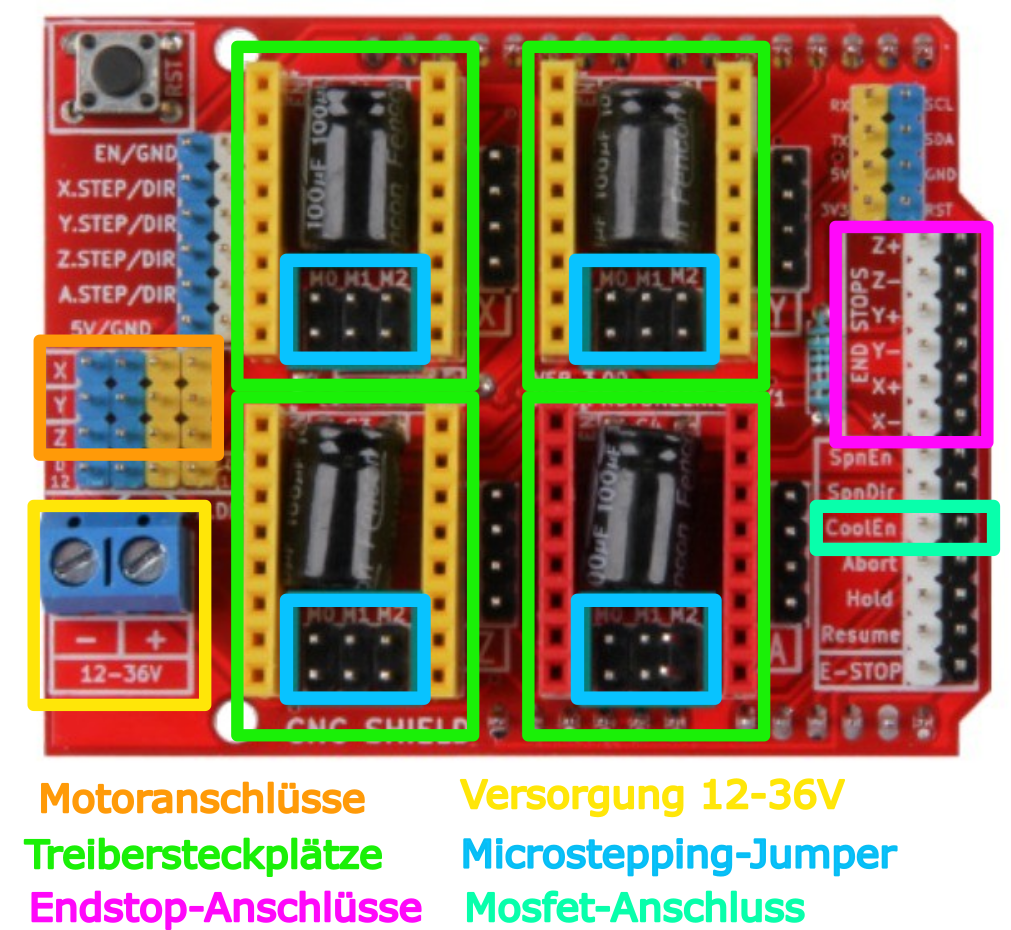
\includegraphics[width=0.85\textwidth]{../../Images/General/CNCGrafik.png}
	\caption{Anschlussübersicht des CNC Shield V3}
	\label{fig:CNCShieldAnschluesse}
\end{figure}

\section{Spezifikation}

Die technischen Daten wurden dem Datenblatt und der Anleitung des Herstellers entnommen \cite{JoyIT:CNCShield:Datenblatt} \cite{JoyIT:CNCShield:Anleitung}.

\begin{itemize}
	\item kompatibel mit Arduino Uno
	\item geeignet für GRBL-basierte CNC-Anwendungen
	\item Steckplätze für bis zu vier Schrittmotortreiber
	\item Achsausgänge für X, Y, Z und A
	\item Anschlüsse für Schrittmotoren
	\item Anschlüsse für Endschalter
	\item Einstellung der Mikroschrittauflösung über Jumper
	\item Anschluss für externe Motorspannung
\end{itemize}

Das CNC Shield erzeugt selbst keine Motorleistung. 
Die Leistung für die Schrittmotoren wird über die eingesetzten Treibermodule bereitgestellt. 
Die Motorspannung wird über die Schraubklemmen des Shields eingespeist und an die Motortreiber verteilt.

\section{Bibliothek}

Für die grundlegende Ansteuerung des CNC Shield V3 wird keine zusätzliche Arduino-Bibliothek benötigt. 
Die Steuerung der Schrittmotortreiber erfolgt über digitale Ausgangssignale des Mikrocontrollers. 
Dabei werden die STEP-, DIR- und ENABLE-Signale direkt über Standardfunktionen der Arduino-IDE erzeugt.

Im späteren Betrieb des CNC-Hot-Wire-Foam-Cutters kann die Bewegungssteuerung durch GRBL erfolgen. 
GRBL erzeugt aus G-Code-Befehlen die notwendigen Schritt- und Richtungssignale für die angeschlossenen Schrittmotortreiber.

Zur direkten Steuerung werden die Funktionen \PYTHON{pinMode()}, \PYTHON{digitalWrite()}, \PYTHON{delay()} und \PYTHON{delayMicroseconds()} verwendet. 
Mit \PYTHON{pinMode()} werden die verwendeten Pins als Ausgänge konfiguriert. 
Mit \PYTHON{digitalWrite()} werden die Zustände der STEP-, DIR- und ENABLE-Pins gesetzt. 
Die Funktion \PYTHON{delayMicroseconds()} bestimmt die Zeit zwischen den Schrittimpulsen und damit die Drehgeschwindigkeit des Motors.

\section{Beispiel}

Dieses Beispiel zeigt, wie eine einzelne Achse des CNC Shield V3 über den Arduino angesteuert werden kann. 
Dabei wird der X-Achsen-Ausgang verwendet. 
Der Test dient dazu, die grundlegende Funktion des Shields, des eingesetzten Motortreibers und des angeschlossenen Schrittmotors zu überprüfen.

\subsection{Montage}

Das CNC Shield V3 wird auf den Arduino Uno aufgesteckt. 
Anschließend wird ein A4988-Schrittmotortreiber in den Steckplatz der X-Achse eingesetzt. 
Dabei muss auf die korrekte Ausrichtung des Treibermoduls geachtet werden, da eine falsche Orientierung den Treiber beschädigen kann \cite{JoyIT:CNCShield:Anleitung}.

Der Schrittmotor wird an den Motoranschluss der X-Achse angeschlossen. 
Die externe Motorspannung wird über die Schraubklemmen des CNC Shields bereitgestellt. 
Vor dem Einschalten muss die Strombegrenzung des eingesetzten Motortreibers eingestellt werden.

\begin{figure}[htbp]
	\centering
	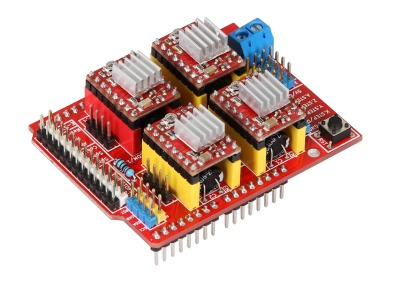
\includegraphics[width=0.75\textwidth]{../../Images/General/CNCKit.jpeg}
	\caption{CNC Shield V3 mit eingesetzten A4988-Schrittmotortreibern}
	\label{fig:CNCShieldA4988Montage}
\end{figure}



\subsection{Erklärung des Beispiel-Codes}

Im Beispiel werden zunächst die Pins für \PYTHON{X\_STEP}, \PYTHON{X\_DIR} und \PYTHON{EN} definiert. 
In der Funktion \PYTHON{setup()} werden diese Pins mit \PYTHON{pinMode()} als Ausgänge konfiguriert. 
Anschließend wird der ENABLE-Pin mit \PYTHON{digitalWrite(EN, LOW)} aktiviert, da der Treiber bei einem LOW-Signal eingeschaltet ist.

In der Funktion \PYTHON{loop()} wird am STEP-Pin ein periodisches Signal erzeugt. 
Dazu wird \PYTHON{X\_STEP} zuerst auf \PYTHON{HIGH} und anschließend wieder auf \PYTHON{LOW} gesetzt. 
Zwischen den Signalwechseln sorgt \PYTHON{delayMicroseconds()} für eine kurze Pause. 
Jeder vollständige Impuls bewegt den Motor um einen Schritt beziehungsweise Mikroschritt weiter.

\subsection{Code}

Der folgende Code prüft die Grundfunktion des CNC Shield V3. 
Die X-Achse wird kontinuierlich in eine Richtung bewegt. 
Dadurch können die Motorspannung, die Treiberorientierung, der Motoranschluss und das STEP-Signal überprüft werden.

{
	\captionof{code}{Einfacher Funktionstest des CNC Shield V3}
	\label{Code:CNCShieldSimpleStep}
	\ArduinoExternal{}{../../Code/CNCShieldSimpleStep/CNCShieldSimpleStep.ino}
}

\subsection{Dateien}

\begin{itemize}
	\item CNCShieldSimpleStep.ino
	\item CNCShieldAxisDemo.ino
	\item CNCShieldFunctionTest.ino
\end{itemize}

\section{Kalibrierung}

Vor dem Betrieb des CNC Shield V3 müssen die eingesetzten Schrittmotortreiber eingestellt werden. 
Besonders wichtig ist dabei die Strombegrenzung des A4988-Treibers. 
Eine zu hohe Einstellung kann zu starker Erwärmung oder zur thermischen Abschaltung führen. 
Eine zu niedrige Einstellung kann dagegen dazu führen, dass der Motor unter Last Schritte verliert.

Die Einstellung erfolgt über das Potentiometer auf dem jeweiligen Motortreibermodul. 
Laut Herstelleranleitung wird die Referenzspannung mit einem Multimeter gemessen und über das Potentiometer angepasst \cite{JoyIT:CNCShield:Anleitung}. 
Dabei muss vorsichtig gearbeitet werden, da die Einstellung direkten Einfluss auf den maximalen Motorstrom hat.

Zusätzlich wird die Mikroschrittauflösung über Jumper unterhalb der Motortreiber eingestellt. 
Für den CNC-Hot-Wire-Foam-Cutter ist eine gleichmäßige Achsbewegung wichtig. 
Daher ist eine feinere Mikroschrittauflösung sinnvoll, sofern der Motor dabei zuverlässig läuft und keine Schritte verliert.

\section{Einfache Anwendung}

Die einfache Anwendung stellt eine projektbezogene Achsbewegung nach. 
Dabei bewegen sich X- und Y-Achse langsam in Schneidrichtung und anschließend schneller zurück. 
Das Beispiel dient zur Demonstration einer kontrollierten Vorschubbewegung, wie sie beim CNC-Hot-Wire-Foam-Cutter benötigt wird.

Im Programm werden die Funktionen \PYTHON{moveAxis()} und \PYTHON{moveXY()} verwendet. 
Die Funktion \PYTHON{moveAxis()} erzeugt Schrittimpulse für eine einzelne Achse. 
Mit \PYTHON{moveXY()} werden zwei Achsen gemeinsam bewegt, sodass eine einfache zweiachsige Bewegung simuliert werden kann.

{
	\captionof{code}{Einfache Achsbewegung mit dem CNC Shield V3}
	\label{Code:CNCShieldAxisDemo}
	\ArduinoExternal{}{../../Code/CNCShieldAxisDemo/CNCShieldAxisDemo.ino}
}

\section{Tests}

\subsection{Einfacher Funktionstest}

Beim einfachen Funktionstest wird geprüft, ob eine einzelne Achse grundsätzlich reagiert. 
Dieser Test erfolgt mit dem Programm aus Abschnitt \ref{Code:CNCShieldSimpleStep}. 
Dabei werden die Verdrahtung, die Versorgungsspannung, der verwendete Motortreiber und die Drehrichtung kontrolliert.

\subsection{Test aller Funktionen}

Beim vollständigen Test werden alle vier Achsausgänge des CNC Shields geprüft. 
Die Motoren werden nacheinander beziehungsweise gemeinsam über die STEP-Pins angesteuert. 
Nach einer festgelegten Schrittzahl wird die Drehrichtung gewechselt. 
Zusätzlich wird das ENABLE-Signal getestet.

Im Testprogramm werden die Pins \PYTHON{X\_STEP}, \PYTHON{Y\_STEP}, \PYTHON{Z\_STEP} und \PYTHON{A\_STEP} verwendet. 
Die Richtung wird über \PYTHON{X\_DIR}, \PYTHON{Y\_DIR}, \PYTHON{Z\_DIR} und \PYTHON{A\_DIR} festgelegt. 
Mit \PYTHON{digitalWrite()} werden die Achsen aktiviert und mit \PYTHON{delay()} beziehungsweise \PYTHON{delayMicroseconds()} zeitlich gesteuert.

Während des Tests wird kontrolliert, ob die Achsen korrekt reagieren, ob sich die Richtung ändert und ob sich die Motortreiber nicht übermäßig erwärmen. 
Der Test ersetzt keine vollständige GRBL-Inbetriebnahme, ermöglicht aber eine grundlegende Prüfung der Hardware.

{
	\captionof{code}{Funktionstest aller Achsausgänge des CNC Shield V3}
	\label{Code:CNCShieldFunctionTest}
	\ArduinoExternal{}{../../Code/CNCShieldFunctionTest/CNCShieldFunctionTest.ino}
}

\section{Weiterführende Literatur}

\begin{itemize}
	\item Hehenberger, Peter: \textit{Computerunterstützte Produktion}. Springer Vieweg, 2020. \cite{Hehenberger:2020}
	\item Joy-IT / SIMAC Electronics GmbH: \textit{ARD-CNC-KIT1 Datenblatt}. 2022. \cite{JoyIT:CNCShield:Datenblatt}
	\item Joy-IT / SIMAC Electronics GmbH: \textit{ARD-CNC-KIT1 Anleitung}. 2023. \cite{JoyIT:CNCShield:Anleitung}
\end{itemize}